\documentclass[journal]{IEEEtran}
\usepackage[T1]{fontenc}
\usepackage{mathptmx}
\usepackage{amsmath,amssymb,amsthm}
\usepackage{graphicx,booktabs,multirow,array}
\usepackage{algorithm,algpseudocode}
\usepackage{cite,xcolor,microtype}
\usepackage{xr-hyper}
\usepackage[hidelinks]{hyperref}
\usepackage{stfloats,placeins,flushend}
\newcommand{\method}{\textsc{MAGIC}}
\newcommand{\E}{\mathbb{E}}
\newcommand{\PP}{\mathbb{P}}
\newcommand{\ind}{\mathbf{1}}
\newcommand{\pos}[1]{[#1]_+}
\newcommand{\Dataset}[1]{\texttt{\detokenize{#1}}}
\newtheorem{proposition}{Proposition}
\newtheorem{theorem}{Theorem}
\newtheorem{corollary}{Corollary}
\DeclareMathOperator*{\argmax}{arg\,max}
\graphicspath{{figures/}}
\setlength{\textfloatsep}{10pt plus 2pt minus 2pt}
\setlength{\floatsep}{8pt plus 2pt minus 2pt}
\setlength{\intextsep}{8pt plus 2pt minus 2pt}
\setlength{\emergencystretch}{1em}
\hyphenation{crowd-sourcing cali-bra-tion like-li-hood}
\renewcommand{\topfraction}{.95}
\renewcommand{\dbltopfraction}{.95}
\renewcommand{\textfraction}{.05}
\setcounter{topnumber}{3}
\setcounter{dbltopnumber}{3}
\makeatletter
\setlength{\@fptop}{0pt}
\setlength{\@fpsep}{14pt}
\setlength{\@dblfptop}{0pt}
\setlength{\@dblfpsep}{14pt}
\makeatother
\newcommand{\smalltable}{\footnotesize\setlength{\tabcolsep}{3.5pt}}

\externaldocument[main-]{main}
\renewcommand{\thesection}{S\arabic{section}}
\renewcommand{\thetable}{S\arabic{table}}
\renewcommand{\thefigure}{S\arabic{figure}}
\renewcommand{\theequation}{S\arabic{equation}}
\begin{document}
\title{Supplementary Material for MAGIC: Adaptive Joint Calibration for Utility-Guided Gold Verification in Crowdsourcing}
\author{}\date{}\maketitle
Sections~\ref{app:model} and~\ref{app:implementation} give derivations, default parameters, dataset provenance, and implementation details. Tables~\ref{tab:complete1} and~\ref{tab:complete2} report all 195 dataset--baseline gains. Sections~\ref{app:accounting} and~\ref{app:supporting} describe delivery diagnostics and supporting experiments.
\section{Model Details and Theoretical Examples}\label{app:model}
\subsection{Notation and Default Settings}

Table~\ref{tab:notation} lists the symbols used across the model and the experiments.

\begin{table}[!ht]
\caption{Main notation. Default hyperparameter values are listed in Table~\ref{tab:settings}.}
\label{tab:notation}\centering\smalltable
\begin{tabular}{@{}l>{\raggedright\arraybackslash}p{0.68\columnwidth}@{}}
\toprule
Symbol & Meaning \\
\midrule
\multicolumn{2}{@{}l}{\emph{Problem and economics}} \\
$n$, $C$ & Numbers of tasks and classes \\
$Y_i$ & Unknown reference label of task $i$ \\
$a_i$, $q_i$ & Fixed predicted label and upstream probability vector \\
$r_i$, $c_i$ & Reward for a correct delivery and gold-label price \\
$L_i(a_i,y)$ & Loss of delivering $a_i$ when the truth is $y$ \\
$U_i(y)$ & Utility of an unverified delivery, \eqref{main-eq:utility} \\
$B$, $B_{\rm r}$ & Total and remaining budget \\
$Q_{\rm tr}$ & Prepaid training tasks of the upstream model \\
$H$, $Q_H$ & Paid calibration history and its purchased tasks \\
$R_H$ & Remaining candidate tasks under $H$ \\
$\mu_i(H)$ & Posterior mean utility $\E[U_i(Y_i)\mid H]$ \\
$S(H)$, $T(H)$ & Delivery set and terminal value, \eqref{main-eq:terminal} \\
\midrule
\multicolumn{2}{@{}l}{\emph{Calibration hypotheses}} \\
$\mathcal{H}$, $K$ & Hypothesis bank and its size $K=|\mathcal{H}|$ \\
$p_{hi}(y)$ & Class distribution of task $i$ under hypothesis $h$ \\
$w_h$ & Prior weight of $h$ \\
$p_i^0$ & Initial predictive distribution, \eqref{main-eq:p0} \\
\midrule
\multicolumn{2}{@{}l}{\emph{Context sharing and evidence}} \\
$v$, $I_v$ & Node of the context tree and its tasks \\
$\alpha$, $\beta$ & Prior masses of the independent branch and the pooled explanation \\
$w_{vh}(H)$ & Posterior weight of $h$ at node $v$ \\
$Z_v^{\rm pool}(H)$, $Z_v(H)$ & Pooled and mixture evidence at $v$ \\
$\rho_v(H)$, $\alpha(H)$ & Posterior masses of the pooled explanation at $v$ and the independent branch \\
\midrule
\multicolumn{2}{@{}l}{\emph{Acquisition}} \\
$\Delta_j(H)$ & One-step value of purchasing task $j$, \eqref{main-eq:gain} \\
$I_j(H)$ & Information value of $j$ for the other tasks, \eqref{main-eq:info} \\
$J_{ji}(y;H)$ & Cross moment $\E[\ind\{Y_j=y\}U_i(Y_i)\mid H]$ \\
\bottomrule
\end{tabular}
\end{table}


Table~\ref{tab:settings} lists the default settings of the calibration bank, context mixture, and acquisition rule in Equations~\eqref{main-eq:calibrator}--\eqref{main-eq:p0} and Algorithm~\ref{main-alg:magic}. The confidence-dependent family contains $3\times5\times2=30$ hypotheses, and the confidence-independent family contains $11\times2=22$, giving $K=52$. The prior-sensitivity analysis in the main text varies $\gamma$, $\alpha$, and $\beta$ one at a time while holding the other settings fixed.

\begin{table}[t]
\caption{Default MAGIC settings, shared by all datasets, baselines, and economic settings.}
\label{tab:settings}\centering\smalltable
\begin{tabular}{lll}
\toprule
Symbol & Role & Default \\
\midrule
$\kappa$ & Confidence clipping & $10^{-6}$ \\
$\mathcal{G}_t$ & Calibration slopes & $\{0.5,1,2\}$ \\
$\mathcal{G}_b$ & Calibration offsets & $\{-4,-2,0,2,4\}$ \\
$\lambda_t,\lambda_b$ & Slope and offset regularization & $1/2,\ 1/8$ \\
$\mathcal{P}$ & Constant correctness probabilities & $\{.05,.1,.2,\ldots,.9,.95\}$ \\
$\eta$ & Upstream-residual mass & $0.75$ \\
$\gamma$ & Confidence-independent family mass & $0.25$ \\
$K$ & Number of hypotheses & $52$ \\
$\alpha$ & Independent-branch mass & $0.5$ \\
$\beta$ & Pooled mass at internal nodes & $0.5$ \\
-- & Purchase threshold & $10^{-8}$ \\
\bottomrule
\end{tabular}
\end{table}

\subsection{Degenerate Inputs}
If $\sum_{y\ne a_i}q_i(y)=0$, use a uniform residual distribution. A confidence-independent hypothesis fixes the probability of the predicted label but can still assign task-specific probabilities to other classes. When a nonsingleton tree node contains identical public features, its split alternative assigns independent marginals to its tasks.

\subsection{Evidence under Adaptive Purchases}
Let $H_t$ denote a particular observed history and $\varphi_t(j\mid H_t)$ the action probability under the policy. The likelihood of the history contains products of label likelihoods and action probabilities. Given the same realized history and public inputs, the action factors do not depend on the latent calibration hypothesis. They cancel in Bayes' rule. For a deterministic policy they equal one along the reached path. The conditioning argument assumes that task selection uses public inputs and previously purchased labels.

\subsection{Diagonal Terms in Moment Computation}
For $i=j$, the exact cross moment is $p_j(y)U_j(y)$ because the outcome fixes the utility. The factorization for distinct tasks does not apply on this diagonal. Equation~\eqref{main-eq:computable} excludes it and credits $r_j-c_j$ separately.

\subsection{Decision Margins and Tightness}\label{app:example}
Consider two equally likely outcomes of query $j$ and two remaining tasks. The first task has conditional mean utilities $-0.5$ and $1.5$, and the second has $1$ and $3$. Both conditional means move by one unit around their respective prior means, giving the same covariance-based bound $D=0.5$. For the first task the margin is $m=0.5$, and rejecting after the first outcome saves $0.5$ with probability one half. For the second, $m=2$ and both outcomes preserve delivery. Equation~\eqref{main-eq:bound} gives the exact transfers, $0.25$ and zero.

More generally, equality in the margin bound holds for any finite outcome support if $m=0$ or $A\le m$. For $0<m<A$, it holds exactly when every positive movement $z_y$ on the support equals $A$: for $0<z<A$, $(z-m)_+< z(1-m/A)$. Thus a two-point movement distribution attains the bound regardless of the outcome probabilities.

\section{Implementation and Reproducibility Details}
\label{app:implementation}
\subsection{Prediction Interfaces and Paid Training}
The experiments use the saved prediction arrays in the main release. Each array contains a full-pool probability matrix, fixed labels, stable task identifiers, rewards, prices, loss rows, and public annotation summaries. Reference labels are stored separately. These outputs allow MAGIC to be rerun directly.

Our LAGNN adaptation uses the authors' public implementation, released as the CrowdGNN repository. It uses the first ten tasks as paid training labels and constructs a graph from annotation agreement. Those labels have already influenced its predictions. They consume the same monetary budget and are never queried again or inserted into MAGIC's calibration history. Our TLLC adaptation uses annotation-derived features and sampled training pairs; pair sampling is part of upstream training, not a reduction of MAGIC's task pool. Both adaptations use the annotations available in the study. MACE and GLAD use the authors' publicly released Python implementations; BCC and TIN retain the behavior of their released implementations. LA\_onepass and LA\_twopass preserve their hard-label outputs, with a one-coin confidence adapter based on worker abilities. All utility calculations use the recorded fixed label even when it differs from the probability-vector maximizer.

\subsection{Dataset Provenance and Coverage}\label{app:data}
Sources for Bird and Web are~\cite{welinder2010multidimensional} and~\cite{zhou2012learning}, respectively. The CF pools are described in~\cite{venanzi2014community,venanzi2015activecrowdtoolkit}, Senti and fej2013 in~\cite{josephy2014workshops}, and the three ZenCrowd pools in~\cite{demartini2012zencrowd}. Sources for Face and product are~\cite{mozafari2014scaling,wang2012crowder,zheng2017truth}. UC is from~\cite{wu2023crowdsourcing}. The multiclass and affective pools (aircrowd6, valence5, and valence7) are described in~\cite{zhang2016multiclass,snow2008cheap}. Table~\ref{tab:datastats} gives annotation density and the underlying utility levels. Relative gain is defined for positive mean reference utility.

\begin{table*}[t]
\caption{Dataset statistics and MAGIC utilities averaged over 13 baselines and three economic settings. Annotations per task divides the annotation count by $n$. Utilities are per task, and reference utility is net utility minus the utility gain in Table~\ref{main-tab:datasets}. ``--'' indicates a nonpositive mean reference utility.}
\label{tab:datastats}\centering\smalltable
\begin{tabular}{lrrrrrrrr}
\toprule
Dataset & $n$ & $C$ & Workers & Annotations & Annotations/task & Reference utility & Net utility & Gain (\%) \\
\midrule
Bird & 108 & 2 & 39 & 4212 & 39.00 & 2.6302 & 2.6149 & -0.58\% \\
CF & 300 & 5 & 461 & 1720 & 5.73 & 2.3698 & 2.8497 & 20.25\% \\
CF\_ & 300 & 5 & 110 & 6025 & 20.08 & 2.2388 & 2.3821 & 6.40\% \\
Face & 584 & 4 & 27 & 5242 & 8.98 & -0.1900 & 0.0601 & -- \\
Senti & 1000 & 5 & 917 & 5503 & 5.50 & 2.5578 & 3.1434 & 22.89\% \\
UC & 100 & 2 & 150 & 2297 & 22.97 & 0.7551 & 0.7551 & 0.00\% \\
Web & 2653 & 5 & 176 & 15539 & 5.86 & 1.9503 & 2.8440 & 45.83\% \\
ZenCrowd\_all & 2040 & 2 & 78 & 20125 & 9.87 & 2.7161 & 2.8534 & 5.06\% \\
ZenCrowd\_in & 2040 & 2 & 25 & 10495 & 5.14 & 1.8502 & 2.0289 & 9.66\% \\
ZenCrowd\_us & 2040 & 2 & 74 & 11155 & 5.47 & 2.6116 & 2.9344 & 12.36\% \\
aircrowd6 & 478 & 6 & 50 & 1473 & 3.08 & 1.9796 & 2.3464 & 18.53\% \\
fej2013 & 576 & 3 & 48 & 2902 & 5.04 & 2.7051 & 3.3448 & 23.65\% \\
product & 8315 & 2 & 176 & 24945 & 3.00 & 3.3807 & 3.8376 & 13.51\% \\
valence5 & 100 & 5 & 38 & 1000 & 10.00 & -2.9908 & -2.4307 & -- \\
valence7 & 100 & 7 & 38 & 1000 & 10.00 & -4.2737 & -0.6231 & -- \\
\bottomrule
\end{tabular}
\end{table*}

\subsection{Economic Settings for the Real Pools}
\label{app:economics}
Each economic seed $s\in\{20261401,20261402,20261403\}$ generates task payoffs deterministically from a SHA-256 hash of the seed, dataset, task identifier, and quantity, so all baselines share identical economics. A public difficulty score $d_i\in[0,1]$ averages normalized vote entropy, one minus the top-two vote margin, and the entropy of reliability-weighted votes, where worker reliability is leave-one-out plurality agreement shrunk toward the global rate with strength 10; reference labels are not used. With $\mathrm{LN}(m,v)$ denoting a log-normal variable with mean $m$ and coefficient of variation $v$, rewards and gold prices are
\begin{equation}
 r_i=\mathrm{LN}(5,0.1)\,(1+0.5d_i),\qquad c_i=\mathrm{LN}(10,0.1)\,(1+0.5d_i).
\end{equation}
For every incorrect pair $(a,y)$ with $y\ne a$, a loss tier is drawn with probabilities 0.6, 0.3, and 0.1 for means 5, 10, and 100, and $L_i(a,y)=\mathrm{LN}(\text{tier mean},0.1)\,(1+d_i)$. Losses therefore depend on the incorrect class, and about one tenth of incorrect pairs carry a high penalty. Because $r_i$ and $c_i$ share the difficulty factor, $c_i/r_i$ does not depend on difficulty. Across all pools and seeds, rewards range from 3.40 to 10.25, prices from 6.61 to 22.11, $c_i/r_i$ from 1.10 to 3.60 with median 2.00, and wrong-label losses from 3.26 to 267.45 with mean 22.88. The budget is $30$ times the median price of the complete pool.


\subsection{Zero-Variance Handling for BWA/UC}
For UC, the supplied BWA code has both zero variance parameter and zero initial worker error. Its worker-precision update therefore divides by zero. The explicit extension is restricted to binary inputs where every task's annotations are unanimous. Under a common positive denominator floor tending to zero, worker precisions diverge while the finite global prior becomes negligible; each task converges to its unanimous label. The extension returns that label and its one-hot probability vector. It uses annotation agreement, not reference correctness, to identify the boundary.

The release checks floors $10^{-3},10^{-6},10^{-9},10^{-12}$ and unchanged nondegenerate outputs on Bird, CF, and Senti. The three BWA/UC main runs complete under this extension. Table~\ref{tab:bwa} groups settings with identical default outputs. This group comprises MAGIC, direct-only queries, both budget changes, doubled prices, $\gamma=0.375$, $\alpha\in\{0.375,0.625,0.75,0.875,1\}$, and every tested $\beta<1$. Removing the broad hypotheses changes the initial delivery even with zero purchases.

\begin{table}[t]
\caption{BWA on UC, averaged over the three economic settings. Gain uses the corresponding common no-additional-query reference. Queries are actual purchases, with fractional values arising only from averaging.}
\label{tab:bwa}\centering\smalltable
\begin{tabular}{lrrr}
\toprule
Setting & Utility gain & Net utility & Queries \\
\midrule
Default group & 0.0000 & 1.0692 & 0.00 \\
\midrule
Compulsory delivery & -1.3543 & -0.2852 & 3.67 \\
Global sharing & -1.6086 & -0.5395 & 2.67 \\
w/o broad hypotheses & -2.1028 & -1.0337 & 0.00 \\
Budget exhaustion & -1.4649 & -0.3957 & 32.00 \\
$c\times0.5$ & 0.0444 & 1.1135 & 4.33 \\
$\gamma=0.10$ & -0.8604 & 0.2088 & 0.33 \\
$\gamma=0.125$ & -0.5884 & 0.4808 & 0.33 \\
$\gamma=0.50$ & 0.0533 & 1.1224 & 2.00 \\
$\gamma=0.625$ & -0.0239 & 1.0453 & 2.67 \\
$\gamma=0.75$ & -0.5128 & 0.5563 & 3.33 \\
$\gamma=0.875$ & -0.6167 & 0.4524 & 3.00 \\
$\gamma=1$ & -0.8160 & 0.2532 & 3.00 \\
$\alpha=0$ & -1.4452 & -0.3760 & 3.33 \\
$\alpha=0.125$ & -0.8165 & 0.2526 & 3.00 \\
$\alpha=0.25$ & -0.0254 & 1.0437 & 0.67 \\
$\beta=1$ & -0.0088 & 1.0603 & 0.33 \\
\bottomrule
\end{tabular}

\end{table}

\subsection{Numerical Evaluation and Trace Reuse}
The initial main implementation uses the dense backend when its cross-moment tensor fits in 3~GiB and the blocked backend otherwise; the blocked backend scores groups of 128 candidates, and candidates in the same leaf with identical hypothesis distributions share their moment rows and are evaluated once. The auxiliary implementation uses exact rectangular moments, candidate blocks of 512, and a cache threshold of 256 tasks for small subtrees. These numbers control working storage and cache reuse. None truncates the task pool, the feasible candidate set, or the observable context tree. Binary hypotheses that differ only in their residual allocation define identical distributions and can be combined by summing prior masses. This optional exact simplification was checked separately; the retained experiment runs preserve the original hypothesis ordering.

Two settings admit exact prefix reuse. Removing the stop gate preserves every previously selected positive-gain purchase before continuing. Under a reduced budget, if the original maximizer remains affordable, it is still a maximizer over the smaller feasible set. Reuse ends when that condition fails, and all feasible scores are recomputed. If the original stop condition has been reached, restricting the feasible set cannot introduce a positive score. Replayed prefixes still invoke the paid oracle, deduct costs, and update evidence. Twenty-six trajectories were checked against complete rescoring with identical query sequences and final delivery.

The verification records include 25 default trajectory replays in the auxiliary implementation and all auxiliary settings replayed on the full 8,315-task product/TLLC input for the first economic seed. Dense and blocked moments are compared across all auxiliary settings; separate numerical checks test evidence and cross moments. These tests address mathematical and implementation equivalence. The audit additionally checks every configuration, input hash, and paid-query trace. For binary outcomes, the extension recovers the second cross moment from $J_{ji}(1)=\mu_i-J_{ji}(0)$ to reduce repeated computation. Scores near ties or the stopping threshold use the original evaluation. State checks and complete trajectory comparisons verify the equivalence. Multiclass pools use FP64 GPU cross moments. Each of two storage implementations passes nine state checks and four complete trajectory comparisons, supplemented by full traces on five further pools, preserving query and delivery decisions. The comprehensive audit recomputes realized utility, accounting identities, paid-label access, uniqueness of queries, and budget feasibility for all 19,890 reported rows. The 2,334 files in the main-release checksum list remain unchanged, and rerunning the main configuration within the supporting framework reproduces the original query sequences and deliveries.

\section{Ablation Definitions and Comparison References}
\label{app:ablations}
Global-pool-only replaces the entire hierarchy and outer independent mixture with one shared calibrator. No-broad removes the 22 confidence-independent hypotheses and renormalizes the remaining 30. Direct-only acquisition replaces the score by $r_j-c_j-[\mu_j]_+$; purchased labels would still update the joint posterior if a query were made. No-stop retains full gain ranking but continues while any task is affordable, regardless of the sign of its score. Compulsory delivery replaces both lookahead terminal utility and final delivery with delivery of all remaining fixed labels, producing score $r_j-c_j-\mu_j$.

The global-pool control replaces both levels of structural mixing. Compulsory delivery changes the acquisition objective and the terminal action together.

Let $N_v$ be variant $v$'s final net utility, $N_0$ the common default-prior no-query reference, and $N_{v,0}$ the variant's own no-query value. Then
\begin{equation}
 N_v-N_0=(N_{v,0}-N_0)+(N_v-N_{v,0}).
\end{equation}
The first term measures a changed starting decision and the second measures purchases and subsequent delivery relative to that starting decision. Comparing only the second term can favor a variant with a poor starting point. We therefore assess relative performance using $N_v-N_{\rm full}$ and report own-reference gains only for interpretation. In a price scenario, $N_0$ is recalculated with that scenario's training prices; the difference from the original final utility also includes changes in training expenditure.

\begin{table}[t]
\caption{Paired sensitivity details over 195 combinations. Difference and W/T/L compare final utility with default MAGIC. Median gain uses the setting's common reference. Intervals are descriptive cluster-bootstrap intervals.}
\label{tab:intervals}\centering\smalltable
\begin{tabular}{lrrrr}
\toprule
Setting & Difference & 95\% CI & W/T/L & Median gain \\
\midrule
$\alpha=0$ & 0.1035 & [-0.1390, 0.3454] & 117/0/78 & 0.2525 \\
$\gamma=0.10$ & -0.2337 & [-0.5208, -0.0152] & 91/4/100 & 0.0982 \\
$\gamma=0.50$ & 0.0667 & [-0.1075, 0.2743] & 94/0/101 & 0.1434 \\
$\alpha=0.25$ & 0.0853 & [0.0168, 0.1701] & 98/0/97 & 0.1615 \\
$\alpha=0.75$ & -0.1909 & [-0.4007, -0.0448] & 69/18/108 & 0.0168 \\
$\beta=0.25$ & 0.0280 & [-0.0116, 0.0597] & 93/18/84 & 0.1297 \\
$\beta=0.75$ & -0.0095 & [-0.1114, 0.1144] & 65/10/120 & 0.0291 \\
$B=15\tilde c$ & -0.0187 & [-0.0452, 0.0006] & 45/93/57 & 0.0904 \\
$B=60\tilde c$ & 0.0067 & [-0.0069, 0.0218] & 32/132/31 & 0.1274 \\
$c\times0.5$ & 0.5657 & [0.3045, 0.9668] & 188/0/7 & 0.5494 \\
$c\times2$ & -0.3109 & [-0.5662, -0.1348] & 41/16/138 & 0.0000 \\
$\gamma=0.125$ & -0.1095 & [-0.2367, -0.0074] & 88/5/102 & 0.0756 \\
$\gamma=0.375$ & 0.0423 & [-0.0793, 0.1863] & 87/10/98 & 0.1031 \\
$\gamma=0.625$ & 0.0873 & [-0.1659, 0.4239] & 83/0/112 & 0.1041 \\
$\gamma=0.75$ & 0.0702 & [-0.2366, 0.4610] & 89/0/106 & 0.1103 \\
$\gamma=0.875$ & 0.0430 & [-0.3508, 0.4789] & 87/0/108 & 0.1863 \\
$\gamma=1$ & -0.1788 & [-0.7183, 0.3470] & 66/0/129 & -0.0027 \\
$\alpha=0.125$ & 0.1072 & [-0.0107, 0.2537] & 116/0/79 & 0.2429 \\
$\alpha=0.375$ & 0.0727 & [0.0046, 0.1601] & 98/13/84 & 0.1639 \\
$\alpha=0.625$ & -0.0259 & [-0.0642, 0.0038] & 70/18/107 & 0.0664 \\
$\alpha=0.875$ & -0.4358 & [-0.9430, -0.1375] & 53/18/124 & 0.0000 \\
$\alpha=1$ & -0.5767 & [-1.0763, -0.2501] & 42/18/135 & 0.0000 \\
$\beta=0$ & -0.5767 & [-1.0763, -0.2501] & 42/18/135 & 0.0000 \\
$\beta=0.125$ & -0.2876 & [-0.7561, -0.0094] & 77/18/100 & 0.0384 \\
$\beta=0.375$ & 0.0165 & [-0.0119, 0.0450] & 86/23/86 & 0.1426 \\
$\beta=0.625$ & -0.0223 & [-0.0665, 0.0210] & 66/14/115 & 0.0723 \\
$\beta=0.875$ & -0.0240 & [-0.1470, 0.1142] & 63/10/122 & 0.0111 \\
$\beta=1$ & -0.0643 & [-0.1743, 0.0387] & 60/1/134 & 0.0018 \\
\bottomrule
\end{tabular}

\end{table}

\begin{table}[t]
\caption{Acquisition rules run to budget exhaustion. Differences are final net utility per task relative to MAGIC. W/T/L counts wins, ties, and losses across 195 combinations. Intervals use the cluster bootstrap and $p$-values use within-family Holm correction.}
\label{tab:paired}\centering\smalltable\setlength{\tabcolsep}{2pt}
\begin{tabular}{lrrrr}
\toprule
Comparison & Difference & 95\% CI & W/T/L & Holm $p$ \\
\midrule
Decision boundary & -0.2464 & [-0.5594, -0.0160] & 61/0/134 & 0.0996 \\
Random & -0.4260 & [-0.8287, -0.1477] & 38/0/157 & 0.0117 \\
Cost-normalized unc. & -0.6266 & [-0.9609, -0.3393] & 32/0/163 & 0.0117 \\
Vote disagreement & -0.6371 & [-0.9342, -0.3853] & 31/0/164 & 0.0117 \\
Least confidence & -0.7317 & [-1.0554, -0.4545] & 29/0/166 & 0.0117 \\
Margin & -0.7164 & [-1.0401, -0.4418] & 28/0/167 & 0.0068 \\
Entropy & -0.7000 & [-1.0215, -0.4225] & 29/0/166 & 0.0117 \\
\bottomrule
\end{tabular}

\end{table}

\section{Statistical Units and Complete Main Results}
\label{app:statistics}
Let $d_{ebs}$ be a per-task gain for dataset $e$, upstream $b$, and economic realization $s$. The principal observation is $\bar d_{eb}=\frac13\sum_s d_{ebs}$ and the main mean is $\frac1{195}\sum_{e,b}\bar d_{eb}$. For paired differences, the same averaging is applied to variant-minus-full values. The index $s$ denotes economic settings with baseline predictions held fixed.

For the 11 dependence clusters, write $D_g$ for the sum of paired differences in cluster $g$ and $m_g$ for its number of combinations. A bootstrap resample of cluster indices $g_1,\ldots,g_{11}$ produces
\begin{equation}
 \widehat d^*=\frac{\sum_{k=1}^{11}D_{g_k}}{\sum_{k=1}^{11}m_{g_k}}.
\end{equation}
This keeps all observations in a sampled cluster together and preserves combination weighting. The interval uses the empirical 2.5th and 97.5th percentiles of the bootstrap resamples with seed 20261025. Sign-flip inference enumerates $2^{11}$ sign assignments to the cluster sums and compares the absolute signed sum with the observed absolute sum. The null hypothesis assumes cluster-level sign symmetry. Holm correction controls each comparison family under the test assumptions: the five ablations, the seven acquisition rules under each budget mode, and the six context-tree variants.

Table~\ref{tab:seeds} retains all three economic groups separately. Tables~\ref{tab:complete1} and~\ref{tab:complete2} show every averaged main combination, including zero and negative outcomes. Sign classifications use the unrounded values.

\begin{table}[t]
\caption{Economic groups before averaging. }
\label{tab:seeds}\centering\smalltable
\begin{tabular}{lrrrr}
\toprule
Economic seed & Net gain & Positive & Zero & Negative \\
\midrule
20261401 & 0.5537 & 117 & 24 & 54 \\
20261402 & 0.4515 & 111 & 22 & 62 \\
20261403 & 0.7248 & 136 & 20 & 39 \\
\bottomrule
\end{tabular}

\end{table}

\begin{table*}[t]
\caption{Complete main net-utility increments, part I. Values are per task and average three economics.}
\label{tab:complete1}\centering\smalltable
\begin{tabular}{lrrrrrrr}
\toprule
Dataset & BCC & BWA & CrowdFM & LAGNN & DawidSkene & GLAD & GOVERN \\
\midrule
Bird & -0.0150 & -0.2850 & 0.0026 & 0.0000 & 0.0000 & 0.0000 & -0.0157 \\
CF & 0.2000 & 0.3910 & -0.3074 & 0.5355 & 0.2573 & -0.0344 & -0.2291 \\
CF\_ & 0.3997 & 0.4285 & 0.0024 & -0.1619 & -0.1349 & 0.2212 & 0.0673 \\
Face & 0.1678 & 0.1263 & 0.1955 & 0.0511 & 0.9881 & 0.2376 & 0.0099 \\
Senti & 0.0519 & 0.6598 & 0.0590 & 0.8614 & 0.2056 & -0.2118 & 0.6298 \\
UC & 0.0000 & 0.0000 & 0.0000 & 0.0000 & 0.0000 & 0.0000 & 0.0000 \\
Web & 0.0550 & 1.0122 & 0.9350 & 0.4438 & 0.2828 & 0.3250 & 2.5574 \\
ZenCrowd\_all & -0.0244 & 0.2619 & -0.0121 & 0.0146 & 0.2089 & 0.1246 & -0.0082 \\
ZenCrowd\_in & 0.1413 & 0.1680 & 0.0714 & -0.1472 & 0.2267 & -0.0744 & 0.3634 \\
ZenCrowd\_us & 0.0811 & 0.0023 & -0.0125 & 0.0292 & 0.1027 & -0.0255 & 0.1479 \\
aircrowd6 & 0.1580 & 0.0284 & 0.0204 & 0.6263 & 0.4661 & 0.0604 & -0.1045 \\
fej2013 & -0.0238 & 0.0274 & 0.4323 & 0.2639 & 1.0381 & 0.2324 & 0.4356 \\
product & -0.0124 & 0.0152 & 0.0724 & 0.2229 & 0.1058 & 0.0046 & 0.7117 \\
valence5 & 2.3991 & -0.0596 & 0.7179 & 0.0571 & 1.6428 & 0.3547 & -0.3037 \\
valence7 & 9.7230 & 0.5586 & 3.6054 & 0.0991 & 7.4294 & 6.0676 & 0.4430 \\
\bottomrule
\end{tabular}

\end{table*}
\begin{table*}[t]
\caption{Complete main net-utility increments, part II.}
\label{tab:complete2}\centering\smalltable
\begin{tabular}{lrrrrrr}
\toprule
Dataset & LA\_onepass & LA\_twopass & MACE & MajorityVote & TIN & TLLC \\
\midrule
Bird & 0.0000 & 0.0000 & -0.0150 & 0.0703 & -0.0110 & 0.0702 \\
CF & 0.0184 & 0.0327 & 0.3625 & 2.4932 & 2.3180 & 0.2011 \\
CF\_ & -0.1446 & -0.1446 & -0.0235 & 0.7496 & 0.6411 & -0.0370 \\
Face & 0.4225 & 0.6430 & 0.4318 & 0.0165 & 0.0746 & -0.1136 \\
Senti & -0.0702 & 0.0406 & -0.0698 & 2.6326 & 2.6168 & 0.2071 \\
UC & 0.0000 & 0.0000 & 0.0000 & 0.0000 & 0.0000 & 0.0000 \\
Web & 0.6441 & 0.3980 & 0.5192 & 1.7684 & 1.9726 & 0.7051 \\
ZenCrowd\_all & -0.0212 & -0.0455 & -0.0065 & 0.5810 & 0.6435 & 0.0686 \\
ZenCrowd\_in & 0.2702 & 0.2261 & 0.2734 & 0.3416 & 0.3017 & 0.1602 \\
ZenCrowd\_us & -0.0711 & -0.0706 & 0.2334 & 0.5300 & 3.2727 & -0.0231 \\
aircrowd6 & 0.0890 & 0.0883 & -0.1014 & 1.4323 & 1.9788 & 0.0268 \\
fej2013 & 0.4434 & 0.4434 & 0.2948 & 0.4236 & 3.1172 & 1.1881 \\
product & -0.0044 & -0.0013 & 1.4454 & 1.0889 & 1.1306 & 1.1601 \\
valence5 & 0.9731 & 0.9731 & 1.1164 & -0.1166 & -0.1465 & -0.3266 \\
valence7 & 6.4652 & 6.4528 & 5.6864 & 0.0847 & 0.0847 & 0.7579 \\
\bottomrule
\end{tabular}

\end{table*}

\section{Accounting and Diagnostic Definitions}
\label{app:accounting}
Let $S_0$ be the common no-additional-query delivery set, $Q_+$ the additional purchased set, and $S$ the final unqueried delivery set. All exclude prepaid training tasks. Writing $u_i=U_i(Y_i)$ for offline realized utility, define
\begin{align}
 D&=\frac1n\sum_{j\in Q_+}\big(r_j-\ind\{j\in S_0\}u_j\big),\\
 V&=\frac1n\left(\sum_{i\in S\setminus S_0}u_i-
 \sum_{i\in S_0\setminus(S\cup Q_+)}u_i\right),\\
 C_+&=\frac1n\sum_{j\in Q_+}c_j.
\end{align}
The exact identity is $N-N_0=D+V-C_+$. The direct term measures gold delivery relative to what the reference would have delivered on purchased tasks. The other-task term measures changes on tasks that remain unqueried. It may include changed initial decisions in prior-changing ablations. This decomposition follows the realized decisions and their costs. The ratio 82.94\% is the ratio of the aggregate other-task gain to aggregate gross gain.

For each full-MAGIC run, let $A$ be its final unqueried set. The multiclass Brier score is
\begin{equation}
 \operatorname{Brier}(p)=\frac1{|A|}\sum_{i\in A}\sum_{y=1}^{C}
 (p_i(y)-\ind\{Y_i=y\})^2.
\end{equation}
It is not divided by $C$. Fixed-label ECE partitions $p_i(a_i)$ into ten equal-width bins and sums each bin's frequency times the absolute difference between mean confidence and empirical fixed-label correctness. Upstream, initial-prior, and final-posterior scores use the identical $A$ within each run. Reported means weight runs equally. Both measures are computed on the adaptively selected remaining tasks.

Learning curves count additional verification steps, excluding prepaid training. Every prefix mean uses all 585 runs. A run that has already stopped contributes its last realized value; an inactive run contributes zero gain. These curves describe progress under the original budget. Budget sensitivity is evaluated separately.

Across all 585 runs, with the terminal state carried forward after stopping, mean cumulative gain reaches 0.2487 after one additional query, 0.4478 after five, 0.5226 after ten, and 0.5633 after twenty. The final gain is 0.5767, so most average improvement occurs early. Of the 7,714 verification steps, 3,122 have negative realized increments, showing variation within individual trajectories.

\subsection{Delivery-Level Diagnostics}
Let $S_0$ be the delivery set before verification and $Q_{\rm tr}$ the paid training set. Define per-task decision headroom by
\begin{equation}
 E_0=\frac1n\left(\sum_{i\in S_0:a_i\ne y_i}L_i(a_i,y_i)+\sum_{i\notin S_0\cup Q_{\rm tr}:a_i=y_i}r_i\right).
\end{equation}
This counts wrong-delivery losses and rewards of correctly predicted but rejected tasks. New error loss concerns incorrect predictions in $S\setminus S_0$; lost correct reward concerns correct predictions in $S_0\setminus(S\cup Q_+)$. The favorable counterparts are recovered correct deliveries and avoided wrong deliveries. Their signed sum equals other-task gain. Task stakes are $\zeta_i=r_i+\frac1{C-1}\sum_{y\ne a_i}L_i(a_i,y)$, and dispersion is their standard deviation divided by their mean. Boundary proximity is the fraction satisfying $|\mu_i(\varnothing)|<0.1\zeta_i$. Economic settings are averaged within combinations before computing quartiles and Spearman associations. Failure-case posteriors replay the recorded paid observations; expected and realized utility sums for newly delivered or rejected sets are divided by the original pool size. Reference labels enter these diagnostics only after decisions have finished.

\begin{table*}[t]
\caption{Five combinations with the lowest utility gains. New error loss and lost correct reward concern delivery changes on unpurchased tasks; utility and cost are per task.}
\label{tab:failures}\centering\smalltable
\begin{tabular}{llrrrrr}
\toprule
Dataset & Baseline & Accuracy & New error loss & Lost correct reward & Query cost & Utility gain \\
\midrule
valence5 & TLLC & 46.00\% & 0.2858 & 0.0386 & 0.4438 & -0.3266 \\
CF & CrowdFM & 88.33\% & 0.3213 & 0.0954 & 0.2542 & -0.3074 \\
valence5 & GOVERN & 29.00\% & 0.3317 & 0.0628 & 0.2059 & -0.3037 \\
Bird & BWA & 75.93\% & 0.2978 & 0.4087 & 0.2825 & -0.2850 \\
CF & GOVERN & 88.00\% & 0.2329 & 0.0059 & 0.2046 & -0.2291 \\
\bottomrule
\end{tabular}

\end{table*}

\section{Supporting Experiments}
\label{app:supporting}
Unless stated otherwise, supporting runs read the frozen main-release inputs, verify their hashes, and use the averaging and cluster inference of Section~\ref{main-sec:protocol}. A run denotes one input (dataset, baseline, and economic seed) under one experimental condition; when several acquisition rules are compared, all of them are evaluated within the same run on that input.

The auxiliary grid contains 34 configurations: the default, five ablations, 24 one-factor prior settings (eight non-default values each of $\gamma$, $\alpha$, and $\beta$), two budgets, and two price multipliers. Together they comprise 19,890 runs including the 585 main runs (6,630 combinations after averaging economics). The supporting study adds 35,035 completed runs: 3,276 subsample the six largest pools, 520 use synthetic pools, and the remainder reuse the 585 frozen inputs. Single-process timing is measured separately.

\subsection{Alternative Acquisition Rules}
Seven rules select tasks under MAGIC's posterior: random selection (five seeds), least confidence, entropy, margin, uncertainty divided by price, vote disagreement, and a decision-boundary heuristic that selects the task minimizing $|\mu_i(H)|/\zeta_i$, with stake $\zeta_i$ defined in Section~\ref{app:accounting}. With matched queries, each run buys as many new labels as the corresponding MAGIC run; with budget exhaustion, it continues until no task is affordable. Delivery uses MAGIC's posterior and~\eqref{main-eq:terminal}. The Platt pipeline instead fits MAP Platt recalibration with prior $N((1,0),I)$ to purchased labels and delivers by the same utility threshold. The comparison comprises 2,340 runs: the 585 main inputs under four conditions (MAGIC's posterior or the Platt pipeline, each with matched queries or budget exhaustion), and each run evaluates all eleven rule trajectories.

\subsection{Published Acquisition Methods}
Three acquisition principles cited in the main text are adapted to paid gold verification on the 585 main inputs. \emph{Opt-KG} (Chen et al.) keeps a Dirichlet posterior with parameters one plus the vote counts for each task; the optimistic knowledge gradient of revealing the label is $1-\max_c I_c$, where $I_c$ is the posterior probability that class $c$ has the largest share, computed exactly for two classes and with 4,000 Monte Carlo draws otherwise. Delivery uses either this vote posterior or MAGIC's posterior. \emph{Optimistic utility} applies the same optimism to MAGIC's exact one-step gain, replacing the expectation over the outcome by its maximum, and stops when this optimistic gain is at most $10^{-8}$. \emph{Liu Local+Global} (Liu et al.) applies the A-optimal greedy rule of their Eq.~(5) to the correctness indicators $z_k$ of the upstream labels, scoring $\mathrm{Var}(z_j)+\sum_{k\ne j}\mathrm{Var}_{y}\,\E[z_k\mid Y_j=y]$ exactly under MAGIC's joint posterior; in the Gaussian case this coincides with the original criterion. \emph{Liu Local} keeps only $\mathrm{Var}(z_j)$, as in their Eq.~(7). \emph{Kapoor VOI} (Kapoor et al.) scores $r_j-c_j+\E_{z_j}\big[\sum_{k\ne j}\pos{\mu_k\mid z_j}\big]-\sum_k\pos{\mu_k}$ under a MAP logistic calibrator on the public context features, refitted exactly for both outcomes, over the 128 tasks closest to the delivery threshold, and stops when the score is at most $10^{-8}$. The advisor-selection methods MADDM and its cautious extension are not included, because their actions choose among imperfect advisors for individual binary decisions rather than selecting tasks for trusted labels.

Each rule follows one deterministic trajectory until budget exhaustion; results at MAGIC's query count and under a rule's own stopping condition are exact prefixes of that trajectory, which was confirmed against separate runs on six inputs. Expected gains recomputed from the joint moments agree with MAGIC's native scores to within $7\times10^{-13}$. The study comprises 1,755 runs: the 585 main inputs in three computation groups, each evaluating one or more rule trajectories.

\subsection{Joint Loss and Price Grid}
The loss multiplier changes every wrong-label loss and the price multiplier changes all verification prices, including those of prepaid training tasks. The original monetary budget is held fixed. Each of the 20 cells has its own no-query reference at the corresponding loss and price levels. The default cell reuses the 585 main runs, leaving $19\times585=11{,}115$ additional runs. The cheaper-gold comparisons reuse overlapping settings. The main article reports the cellwise gains and the multiplicity-adjusted tests.

\subsection{Cheaper and Noisy Gold Labels}
Cheaper gold labels multiply all prices by 0.1 or 0.25 with the monetary budget fixed, and the reference is recomputed with the new training prices. Random selection (three seeds) and cost-normalized uncertainty use MAGIC's posterior with matched queries or budget exhaustion (1,170 runs: the 585 main inputs at two price multipliers, each run evaluating MAGIC and the eight comparison trajectories).

For $\varepsilon\in\{5\%,10\%,20\%\}$, whether each task's gold label is corrupted is fixed before purchasing, so corruption does not depend on query order; prepaid training labels remain clean. The loss charged when an incorrect verified label is delivered (the task's mean, zero, or maximum wrong-label loss) affects evaluation only. With zero loss, MAGIC gains 0.5414, 0.4493, and 0.3502 per task. Random selection (three seeds), least confidence, and the decision-boundary heuristic buy MAGIC's query count under the same noise (1,755 runs: the 585 main inputs at three noise rates, each run evaluating MAGIC and the five comparison trajectories).

\subsection{Noise-Aware Likelihood}
The noise-aware variant assumes that a returned gold label equals the reference label with probability $1-\varepsilon_m$ and is otherwise uniform over the other $C-1$ classes. Only the observation channel changes: the hypothesis probabilities used to score candidate outcomes and to update evidence become $p_{hj}(y)(1-\varepsilon_m)+(1-p_{hj}(y))\,\varepsilon_m/(C-1)$, while terminal utilities keep the noise-free label distribution, so initial delivery is unchanged; every run asserts this. The direct value of delivering a purchased label becomes $(1-\varepsilon_m)r_j$ minus $\varepsilon_m$ times the task's mean wrong-label loss. The corruption streams are those of the noisy-gold experiment, and $\varepsilon_m=0$ reproduces the original MAGIC query sequences and utilities exactly. Settings cross $\varepsilon\in\{5\%,10\%,20\%\}$ with $\varepsilon_m\in\{\varepsilon/2,\varepsilon,2\varepsilon\}$ and add $\varepsilon=0$ with $\varepsilon_m\in\{5\%,10\%\}$ to measure the cost without noise (6,435 runs).

\subsection{Synthetic Pools}
Each pool has 500 tasks, rewards drawn from $U(5,9)$, price-to-reward ratios from $U(1.1,3.0)$, wrong-label losses from a log-normal distribution with median 15 and log-scale deviation 0.8, and a budget of 30 median prices. In the correctly specified setting, labels are sampled exactly from the joint law of the default MAGIC prior for 100 pools with two classes and 100 with three. In the misspecified setting, a Dawid--Skene-type simulation assigns tasks to five latent groups whose effects $\delta_g\sim N(0,\sigma^2)$ shift each worker's accuracy logit, with default $\sigma=1$, 20\% spammers, and $R=5$ votes per task. One factor varies at a time: $\sigma\in\{0,0.5,2\}$, spammer rate $\in\{0,0.4\}$, or $R\in\{3,7\}$. Smoothed majority vote and Dawid--Skene EM provide upstream predictions from the same votes, with 20 replicates per setting (520 runs in total).



Figure~\ref{main-fig:synthetic} in the main article reports the simulated gains. The other-task share of gross gain is lower for Dawid--Skene than for majority vote in seven of eight settings.

\subsection{Task-Value Dispersion}
For positive rewards and wrong-label losses within a pool, $\log x'=\overline{\log x}+\lambda(\log x-\overline{\log x})$, followed by a rescaling that restores the arithmetic mean. Prices, predictions, and budgets are unchanged, and $\lambda=1$ reproduces the main runs (1,755 new runs). The mean coefficient of variation of task stakes is 0, 0.40, and 1.53 for $\lambda=0$, 0.5, and 1.5. At $\lambda=0$ the gain concentrates on fewer combinations: 104 improve and 65 decline, compared with 135 and 42 at $\lambda=1$.

\subsection{Two-Step Lookahead}
For the six pools with at most 300 tasks (Bird, CF, CF\_, UC, valence5, and valence7; 234 runs, 78 combinations, four clusters), the two-step value is
\begin{equation}
 V_2(j)=\Delta_j(H)+\sum_y P(Y_j=y\mid H)\,\pos{\max_{j'}\Delta_{j'}\big(H\cup\{(j,y)\}\big)},
\end{equation}
evaluated for the 20 tasks with the largest one-step gain, where $j'$ ranges over tasks still affordable after paying for $j$. The policy buys the maximizer when $V_2>10^{-8}$ and replans. It makes 4.40 new queries on average, compared with 3.76, and gains 0.8716 compared with 0.8031. With four clusters the smallest attainable sign-flip $p$ is 0.125; the observed value is 1.00, whereas a Wilcoxon test ($p=0.0044$) indicates that more combinations favor the one-step rule. In the 66 main-design runs where the one-step rule makes no purchase, the two-step rule buys labels in 60 runs (0.95 per run on average) and changes utility by $-0.0400$ per task on average, with 3 runs improving, 6 tied, and 57 declining.

\subsection{Context-Tree Variants}
Random trees replace the public splitting features with random features (three seeds). Feature-removal variants rebuild the tree without confidence, margin, annotation count, entropy, or class indicators. The hypothesis bank, priors, independent branch, and node pooling are unchanged, and each run asserts that its initial delivery matches the full model (4,680 runs).

\subsection{Runtime}
Timing uses one process with single-threaded BLAS and no concurrent jobs. Subpools of product (two classes) and Web (five classes) range from 250 tasks to the full pool. Fig.~\ref{fig:runtime} reports the mean time per acquisition step. Log--log slopes are 1.46, 1.88, 1.34, and 0.88 on product for the blocked, dense, exact-binary, and GPU backends, and 2.01, 1.96, and 0.58 on Web for the blocked, dense, and GPU backends. The CPU slopes do not exceed the quadratic pair interactions of exact moment computation, and the lower slopes on product reflect linear overhead at these sizes; the GPU slopes reflect incomplete device utilization at these sizes rather than a lower complexity. The dense CPU backend exceeds memory on the full product pool, where the blocked backend peaks at 0.5~GB and the GPU uses a 9.4~GB memory pool. On the full Web pool, a step takes 1.02~s on the blocked CPU backend and 0.031~s on the GPU.  At the largest pools, the GPU backend is 3.9 times faster than the fastest CPU backend on product and 25.8 times faster on Web (Fig.~\ref{fig:runtime}c).

\begin{figure*}[t]
\centering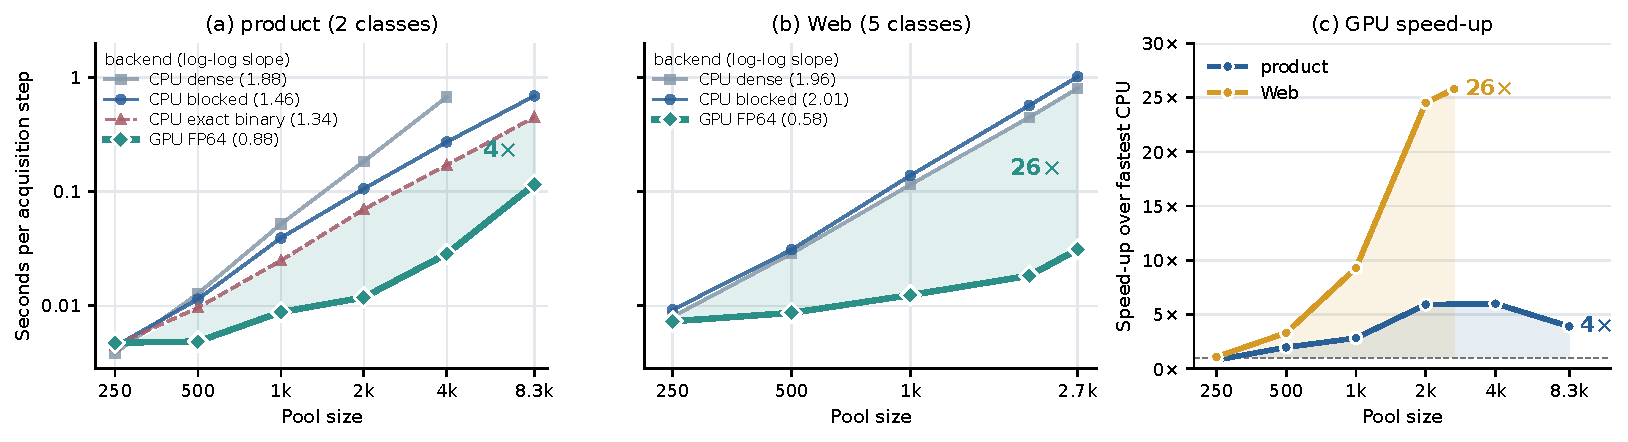
\includegraphics[width=\textwidth]{runtime.pdf}
\caption{Mean time per acquisition step versus pool size, measured in a single process. (a)--(b)~Log--log curves for each backend on product (two classes) and Web (five classes); numbers in the legend are log--log slopes, and the shaded band between the GPU and the fastest CPU backend marks the speed-up. (c)~GPU speed-up over the fastest CPU backend at each pool size.}
\label{fig:runtime}
\end{figure*}

\subsection{Rank-Based Cross-Check}
Treating the 195 combinations as independent, Wilcoxon signed-rank tests with Holm correction give $p\le2.7\times10^{-5}$ for the main gain and all five ablations, each in the direction of the cluster analysis. Budget exhaustion is significant under this test but not under the cluster test ($p=0.1523$), which remains the primary analysis.

\bibliographystyle{IEEEtran}
\bibliography{references}

\end{document}
